\documentclass{standalone}

\usepackage{pgfplots,tikz,amsmath}
\begin{document}
		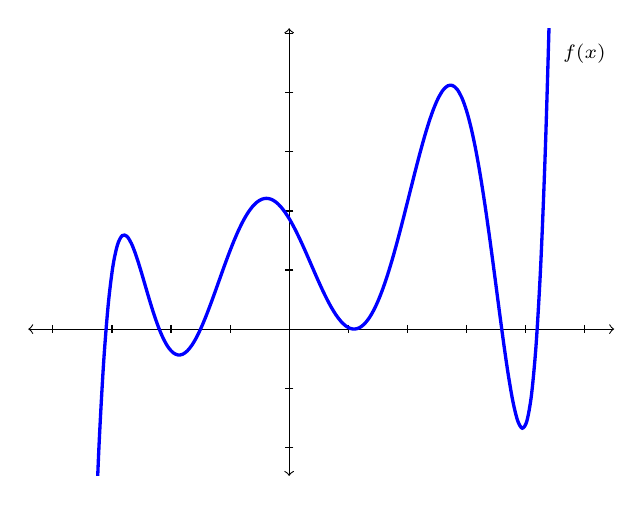
\begin{tikzpicture}[scale=0.75]
			[line cap=round,line join=round,>=triangle 45,x=1.0cm,y=1.0cm] 
			\draw[<->,color=black] (-4.418087504107611,0.0) -- (5.504275777242757,0.0); \foreach \x in {-4.0,-3.0,-2.0,-1.0,1.0,2.0,3.0,4.0,5.0} 
			\draw[shift={(\x,0)},color=black] (0pt,2pt) -- (0pt,-2pt); 
			\draw[<->] (0.0,-2.486833997057605) -- (0.0,5.09438316608086); \foreach \y in {-2.0,-1.0,1.0,2.0,3.0,4.0,5.0} 
			\draw[shift={(0,\y)},color=black] (2pt,0pt) -- (-2pt,0pt); 
			\clip(-4.418087504107611,-2.486833997057605) rectangle (5.504275777242757,5.09438316608086); 
			\draw[color=blue, very thick,smooth,samples=100,domain=-3.3:4.5]
			plot(\x,{((\x)-1.1)^(2.0)*((\x)-3.6)*((\x)+1.5)*((\x)-4.2)*((\x)+2.2)*((\x)+3.1)/100.0});
			\begin{scriptsize}
				\draw[color=black] (5,4.671245463952202) node {$f(x)$};
			\end{scriptsize}
		\end{tikzpicture}
		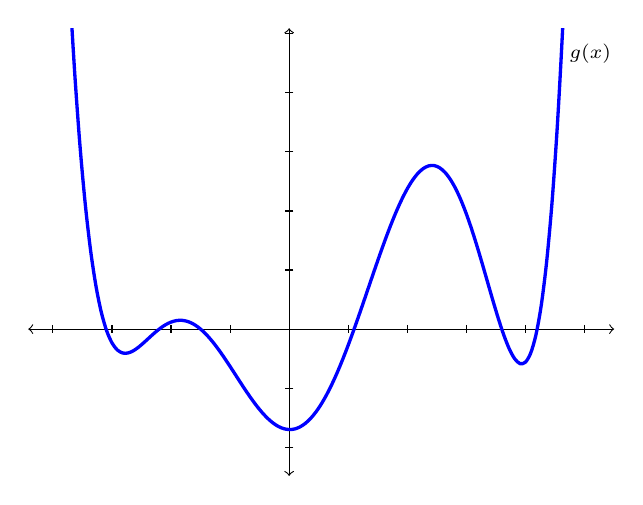
\begin{tikzpicture}[scale=0.75]
			[line cap=round,line join=round,>=triangle 45,x=1.0cm,y=1.0cm] 
			\draw[<->,color=black] (-4.418087504107611,0.0) -- (5.504275777242757,0.0); \foreach \x in {-4.0,-3.0,-2.0,-1.0,1.0,2.0,3.0,4.0,5.0} 
			\draw[shift={(\x,0)},color=black] (0pt,2pt) -- (0pt,-2pt); 
			\draw[<->,color=black] (0.0,-2.486833997057605) -- (0.0,5.09438316608086); \foreach \y in {-2.0,-1.0,1.0,2.0,3.0,4.0,5.0} 
			\draw[shift={(0,\y)},color=black] (2pt,0pt) -- (-2pt,0pt); 
			\clip(-4.418087504107611,-2.486833997057605) rectangle (5.504275777242757,5.09438316608086); 
			\draw[color=blue, very thick,smooth,samples=100,domain=-4:5]
			plot(\x,{((\x)-1.1)*((\x)-3.6)*((\x)+1.5)*((\x)-4.2)*((\x)+2.2)*((\x)+3.1)/100.0});
			\begin{scriptsize}
				\draw[color=black] (5.1,4.671245463952202) node {$g(x)$};
			\end{scriptsize}
		\end{tikzpicture} 
\end{document}
